\section{$n$维球的体积与表面积}\label{sec:N-sphere}
	这一节我们研究$n$维球的体积与表面积问题.我们在这里说的“$n$维球”指的是嵌入$\mathbb{R}^n$中的球,通常用符号$S^{n-1}$表示,也就是说球的边界是$n-1$维的.我们先给出结论,然后去证明它.
	\begin{theorem}
		一个半径为$r$的$n$维球的体积$V_n(r)$、表面积$S_n(r)$分别为
		\begin{eqnarray}\label{eq:V_n(r),S_n(r)}
			V_n(r)&=&\frac{\pi^{\frac{n}{2}}}{\varGamma\left(\frac{n}{2}+1\right)}r^n;\\
			S_n(r)&=&\frac{2\pi^{\frac{n}{2}}}{\varGamma\left(\frac{n}{2}\right)}r^{n-1}.
		\end{eqnarray}
	\end{theorem}
		
	\begin{proof}
		这个问题有一个优雅的解决方案,即使用Gauss 积分.首先我们明确这样一个性质,半径为$r$的$n$维球的体积$V_n(r)$一定正比于$r^n$,比例系数是单位球的体积$V_n(1)$:
		\begin{eqnarray}\label{eq:V_n(r)}
			V_n(r)=V_n(1)r^n. 
		\end{eqnarray}
		我们对(\ref{eq:V_n(r)})微分可以得到表面积满足
		\begin{eqnarray}\label{eq:S_n(r)}
			dV_n(r)=nV_n(1)r^{n-1}dr=S_n(r)dr, 
		\end{eqnarray}
		其中$S_n(r)\equiv =nV_n(1)r^{n-1}$.构造这样一个Gauss型积分
		\begin{eqnarray}\label{eq:Gauss int}
		\int_{\mathbb{R}^n}e^{-r^2}dV_n,
		\end{eqnarray}
		现在我们尝试求出(\ref{eq:Gauss int}).若取坐标系为超球坐标系,则有
		\begin{eqnarray}\label{eq:Gauss int1}
			\int_{\mathbb{R}^n}e^{-r^2}dV_n=nV_n(1)\int_0^{+\infty}r^{n-1}e^{-r^2}dr,
		\end{eqnarray}
		作一个变量替换$u=r^2$,代入得
		\begin{eqnarray*}
			\int_0^{+\infty}r^{n-1}e^{-r^2}dr&=&\frac{1}{2}\int_0^{+\infty}u^{\frac{n}{2}-1}e^{-u}du=\frac{1}{2}\varGamma\left(\frac{n}{2}\right),
		\end{eqnarray*}
		于是
		\begin{eqnarray}\label{eq:Gauss int2}
			\int_{\mathbb{R}^n}e^{-r^2}dV_n(r)=V_n(1)\frac{n}{2}\varGamma\left(\frac{n}{2}\right)=V_n(1)\varGamma\left(\frac{n}{2}+1\right);
		\end{eqnarray}
		若取坐标系为直角坐标系,则有
		\begin{eqnarray}\label{eq:Gauss int3}
			\int_{\mathbb{R}^n}e^{-r^2}dV_n=\int_{\mathbb{R}^n}e^{-\left[(x^1)^2+\cdots+(x^n)^2\right]}dx^1\cdots dx^n=\left(\int_{-\infty}^{+\infty}e^{-x^2}dx\right)^n,
		\end{eqnarray}
		作一个变量替换$u=x^2$,代入得
		\begin{eqnarray*}
			\int_{-\infty}^{+\infty}e^{-x^2}dx=\int_{0}^{+\infty}u^{-\frac{1}{2}}e^{-u}dx=\varGamma\left(\frac{1}{2}\right)=\pi^{\frac{1}{2}},
		\end{eqnarray*}
		于是
		\begin{eqnarray}\label{eq:Gauss int4}
			\int_{\mathbb{R}^n}e^{-r^2}dV_n=\pi^{\frac{n}{2}}.
		\end{eqnarray}
		结合(\ref{eq:V_n(r)}),(\ref{eq:S_n(r)}),(\ref{eq:Gauss int2})以及(\ref{eq:Gauss int4})我们得到
		\begin{eqnarray}
			%V_n(1)&=&\frac{\pi^{\frac{n}{2}}}{\varGamma\left(\frac{n}{2}+1\right)};\notag\\
			V_n(r)&=&\frac{\pi^{\frac{n}{2}}}{\varGamma\left(\frac{n}{2}+1\right)}r^n;\notag\\
			%S_n(1)&=&\frac{2\pi^{\frac{n}{2}}}{\varGamma\left(\frac{n}{2}\right)};\notag\\
			S_n(r)&=&\frac{2\pi^{\frac{n}{2}}}{\varGamma\left(\frac{n}{2}\right)}r^{n-1}.\notag
		\end{eqnarray}
	\end{proof}

	我们可以取单位球$r=1$来研究$V_n(1)$与$S_n(1)$随维数$n$变化的关系,如图\ref{fig:V_n(1)},\ref{fig:S_n(1)}所示.
	\begin{figure}[h]
		\centering
		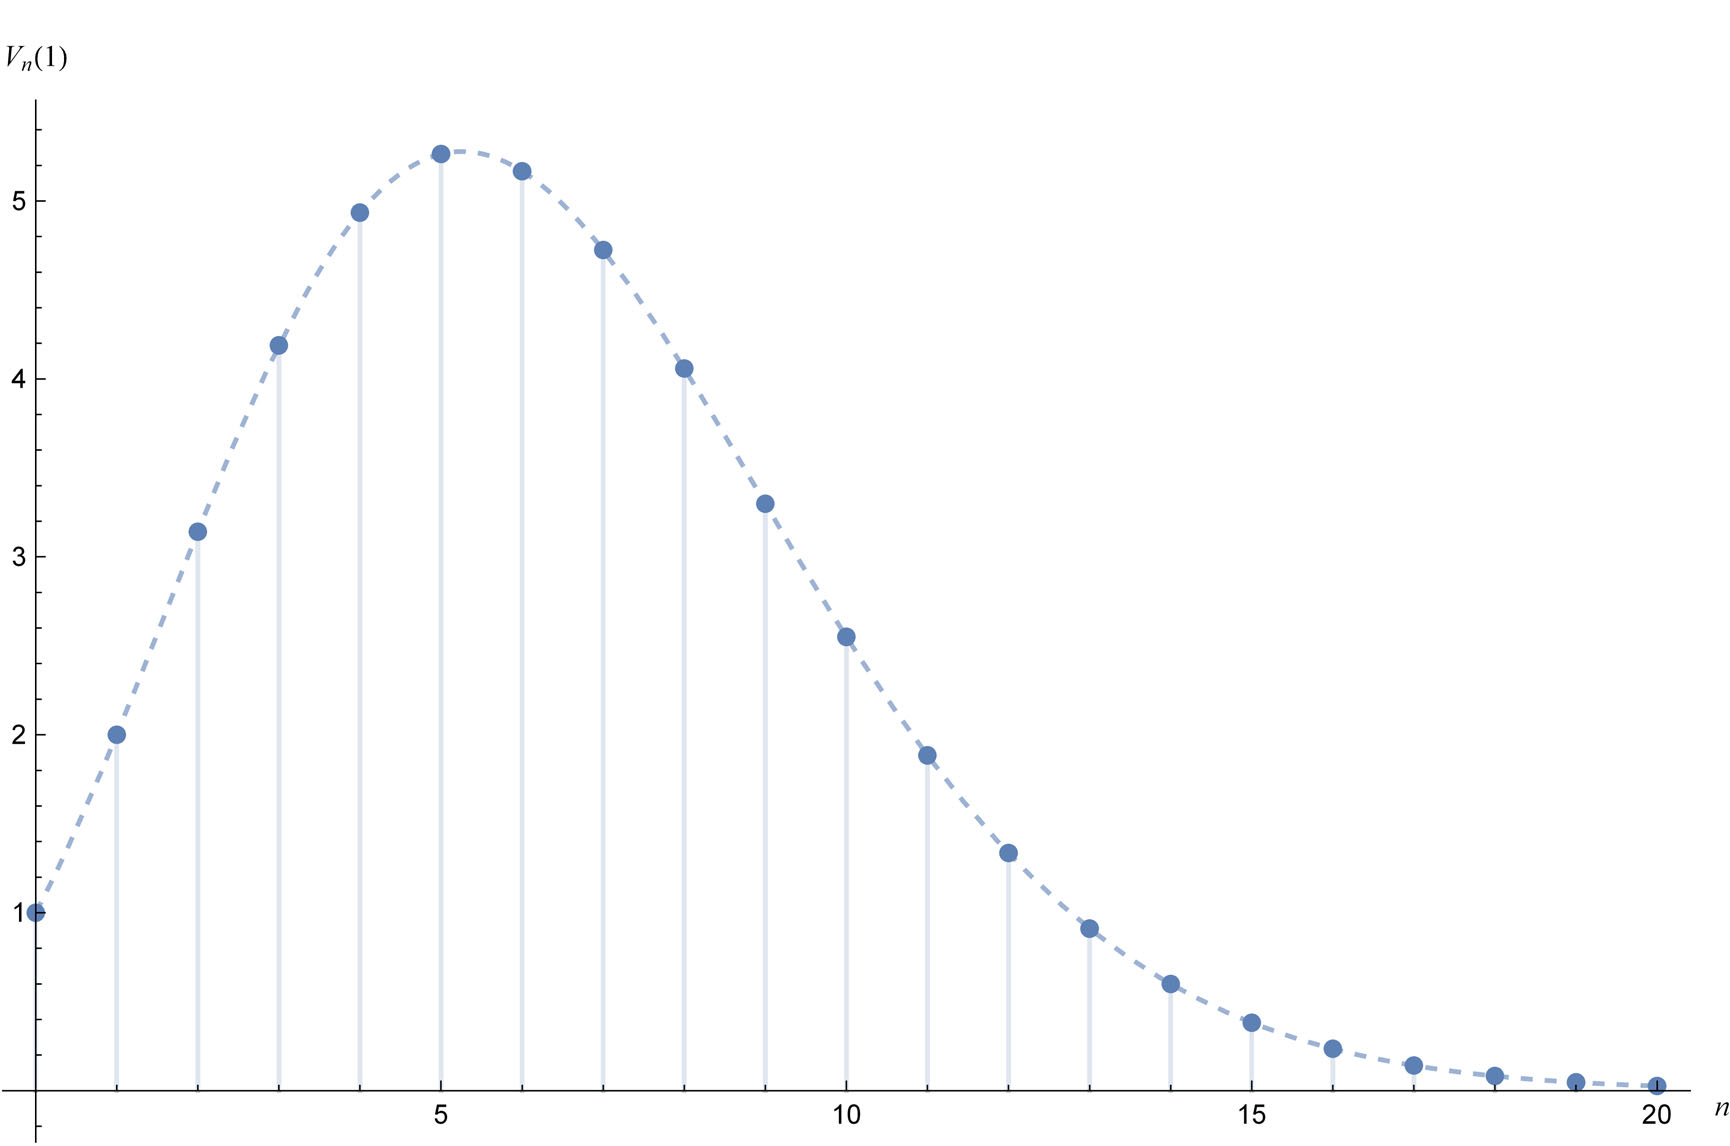
\includegraphics[width=0.75\textwidth]{figures/V_n(1).jpg}
		\caption{$V_n(1)$随$n$的变化关系}\label{fig:V_n(1)}
	\end{figure}

	\begin{figure}[h]
		\centering
		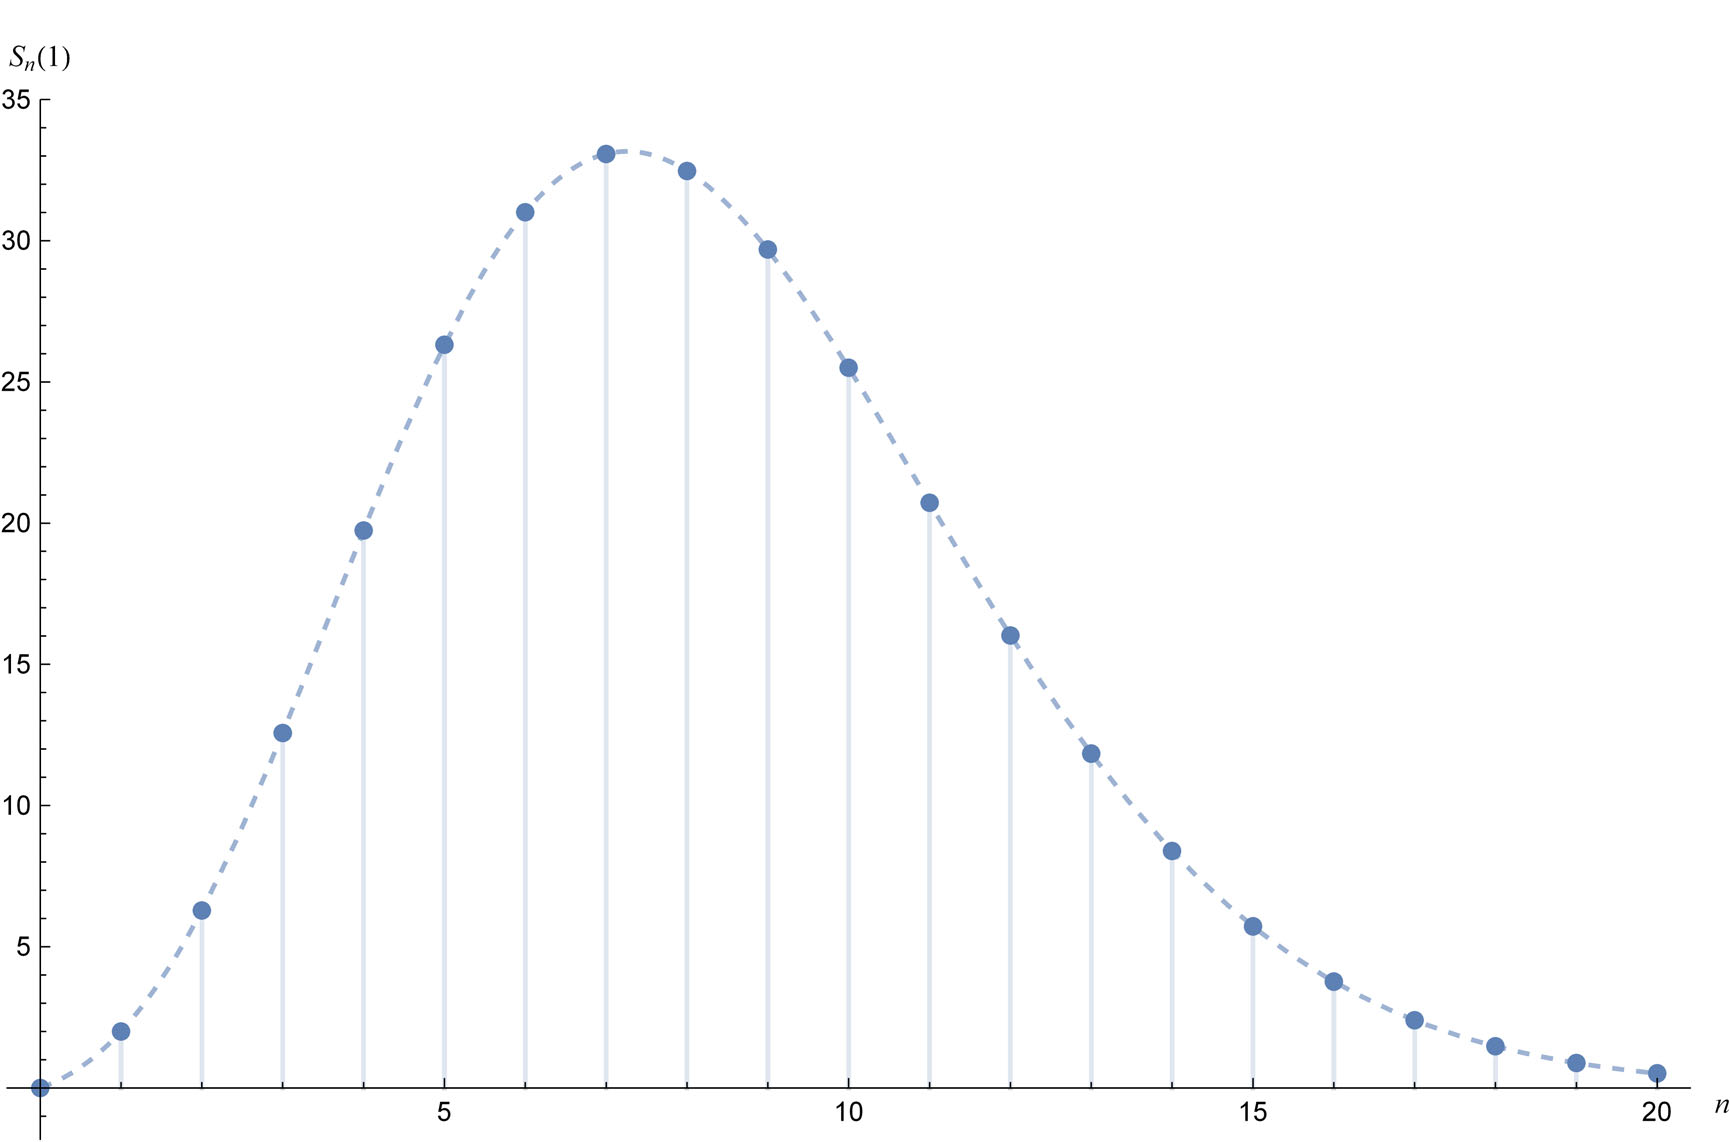
\includegraphics[width=0.75\textwidth]{figures/S_n(1).jpg}
		\caption{$S_n(1)$随$n$的变化关系}\label{fig:S_n(1)}
	\end{figure}
	可以看到,当$n=5$时,单位球的体积最大;当$n=7$时,单位球的表面积最大.而随着维数$n$不断增大,单位球的体积、表面积却在趋于零,这种现象源于Gamma函数的增长速度远大于指数函数.

	高维球还产生了一些有趣的问题,例如高维空间的最密堆积问题.目前这一问题还没有通解.另外,我们还可以引入Hausdorff维数,使得$n$的取值范围从正整数集扩大到实数集,此时又会产生怎样的新问题?
	
	\newpage